% **************************************************
% Document Class Definition
% **************************************************
\documentclass[runningheads]{llncs}

% !TEX root = main.tex
% chktex-file 46

% **************************************************
% Files' Character Encoding
% **************************************************
\PassOptionsToPackage{utf8}{inputenc}
\usepackage{inputenc}
\usepackage[ngerman,english]{babel}
\usepackage{csquotes}

% **************************************************
% Information and Commands for Reuse
% **************************************************
\newcommand{\thesisTitle}{Spectral Graph Approximation}
\newcommand{\thesisName}{Clemens Damke}
\newcommand{\thesisMatNr}{7011488}
\newcommand{\thesisSubject}{Seminar paper}
\newcommand{\thesisDate}{}

\newcommand{\thesisSupervisor}{Vitalik Melnikov}

\newcommand{\thesisUniversity}{Paderborn University}
\newcommand{\thesisUniversityDepartment}{Department of Computer Science}
\newcommand{\thesisUniversityInstitute}{Heinz Nixdorf Institute}
\newcommand{\thesisUniversityGroup}{Intelligent Systems and Machine Learning Group (ISG)}
\newcommand{\thesisUniversityCity}{Paderborn}
\newcommand{\thesisUniversityStreetAddress}{Warburger Straße 100}
\newcommand{\thesisUniversityPostalCode}{33098}



% **************************************************
% Debug LaTeX Information
% **************************************************
%\listfiles


% **************************************************
% Load and Configure Packages
% **************************************************
\usepackage{geometry}
\geometry{
  a4paper,
  % textwidth=13cm,
  % textheight=23cm,
  % heightrounded,   % integer number of lines
  hratio=1:1,      % horizontally centered
  % vratio=1:1,      % vertically centered
}
\renewcommand{\baselinestretch}{1.15}
\usepackage[parfill]{parskip}
\usepackage{float}

% Colors:
\usepackage[usenames, dvipsnames, svgnames, table]{xcolor}

\definecolor{schwarz}{HTML}{000000}
\definecolor{blau}{HTML}{3F6DB1}
\definecolor{rot}{HTML}{EE7993}
\definecolor{gruen}{HTML}{3FB17D}

\usepackage{mathtools}
\usepackage{bm}
\usepackage{bbm}
\usepackage{units}
\usepackage{upgreek}
\newcommand\numberthis{\addtocounter{equation}{1}\tag{\theequation}}

\usepackage{algorithm}
\usepackage[noend]{algpseudocode}

\usepackage{graphicx}
\usepackage{tikz}
\usetikzlibrary{arrows,positioning}
\usetikzlibrary{calc}
\newcommand{\tikzmark}[1]{\tikz[overlay,remember picture] \node (#1) {};} % chktex 1
\usepackage[labelfont=bf]{caption}
\usepackage{subcaption}
\usepackage{wrapfig}

\usepackage{pgfplots}
\usepackage{pgfplotstable}
\pgfplotsset{compat=1.14}
\usepgfplotslibrary{dateplot, statistics}
\pgfplotsset{
    cycle list={blau\\rot\\gruen\\schwarz\\},
}

\usepackage{listings}
\lstset{basicstyle=\ttfamily,breaklines=true}
\usepackage[inline]{enumitem}

\usepackage{amsmath,amssymb}
\usepackage{stmaryrd}
\usepackage{multicol}
\usepackage{pbox}
\usepackage{longtable}
\usepackage{booktabs}
\usepackage{csvsimple}
\usepackage{siunitx}

\usepackage{hyperref}
\hypersetup{% setup the hyperref-package options
    pdftitle={\thesisTitle},    %   - title (PDF meta)
    pdfsubject={\thesisSubject},%   - subject (PDF meta)
    pdfauthor={\thesisName},    %   - author (PDF meta)
    plainpages=false,           %   -
    colorlinks=false,           %   - colorize links?
    pdfborder={0 0 0},          %   -
    breaklinks=true,            %   - allow line break inside links
    bookmarksnumbered=true,     %
    bookmarksopen=true          %
}
\usepackage[nameinlink]{cleveref}
\newcommand{\crefrangeconjunction}{--}

\usepackage[						% use biblatex for bibliography
	backend=bibtex,					% 	- use biber backend (bibtex replacement) or bibtex
	style=numeric,					% 	- use alphabetic (or numeric) bib style
	natbib=true,					% 	- allow natbib commands
	hyperref=true,					% 	- activate hyperref support
	backref=true,					% 	- activate backrefs
	isbn=false,						% 	- don't show isbn tags
	url=false,						% 	- don't show url tags
	doi=false,						% 	- don't show doi tags
	urldate=long,					% 	- display type for dates
	maxnames=3,%
	minnames=1,%
	maxbibnames=5,%
	minbibnames=3,%
	maxcitenames=2,%
	mincitenames=1%
]{biblatex}
\bibliography{bib-refs}

\DeclareCiteCommand{\citenum}
  {}
  {\bibhyperref{\printfield{labelnumber}}}
  {}
  {}


\newcommand{\Dtrain}{\mathcal{D}_{\mathit{train}}}
\newcommand{\Dvalid}{\mathcal{D}_{\mathit{valid}}}
\newcommand{\Dtest}{\mathcal{D}_{\mathit{test}}}
\newcommand{\sourceinline}[2][source]{{\scriptsize\textsc{#1:~\cite{#2}}}}
\newcommand{\source}[2][source]{\null\hfill\sourceinline[#1]{#2}}

% **************************************************
% Document CONTENT
% **************************************************
\begin{document}

% --------------------------
% Front matter
% --------------------------
% !TEX root = ../main.tex
%

\title{\thesisTitle}
\author{\thesisName}
\institute{{\thesisUniversityGroup} \\
{\thesisUniversityInstitute} \\
{\thesisUniversity} \\
{\thesisUniversityStreetAddress} \\
\thesisUniversityPostalCode\ \thesisUniversityCity}

\maketitle

% !TEX root = ../main.tex
%
\begin{abstract}%
	This paper describes how coarsening affects the spectrum of a graph.
	For this the notion of restricted spectral similarity is introduced.
	This similarity measure compares graphs via the distance between their Laplacian's eigenvalues.
	The measure is used to show that the spectral distortion introduced by coarsening is smallest for regular graphs.
\end{abstract}


% --------------------------
% Body matter
% --------------------------

% !TEX root = ../main.tex
% chktex-file 21
% chktex-file 46
\section{Introduction}%
\label{sec:intro}

\pagenumbering{arabic}			% arabic page numbering
\setcounter{page}{1}			% set page counter

With the rise of Big Data applications over the recent years, working with large graph structures also became more important.
Algorithms like PageRank or spectral clustering are commonly used to analyze the web graph or social networks.
In order to run such algorithms on large graphs however, optimizations are required.

For this purpose we will specifically look at \textit{graph coarsening}.
Coarsening reduces the size of a given graph while preserving its overall structure via some notion of graph similarity that will be defined later.
Graph algorithms can then be run on the smaller coarsened graph.
Afterwards the result for the coarsened graph can be iteratively refined to obtain an approximate result for the original graph.
\Cref{fig:intro:overview} illustrates this approach.
\begin{figure}[ht]
	\centering
	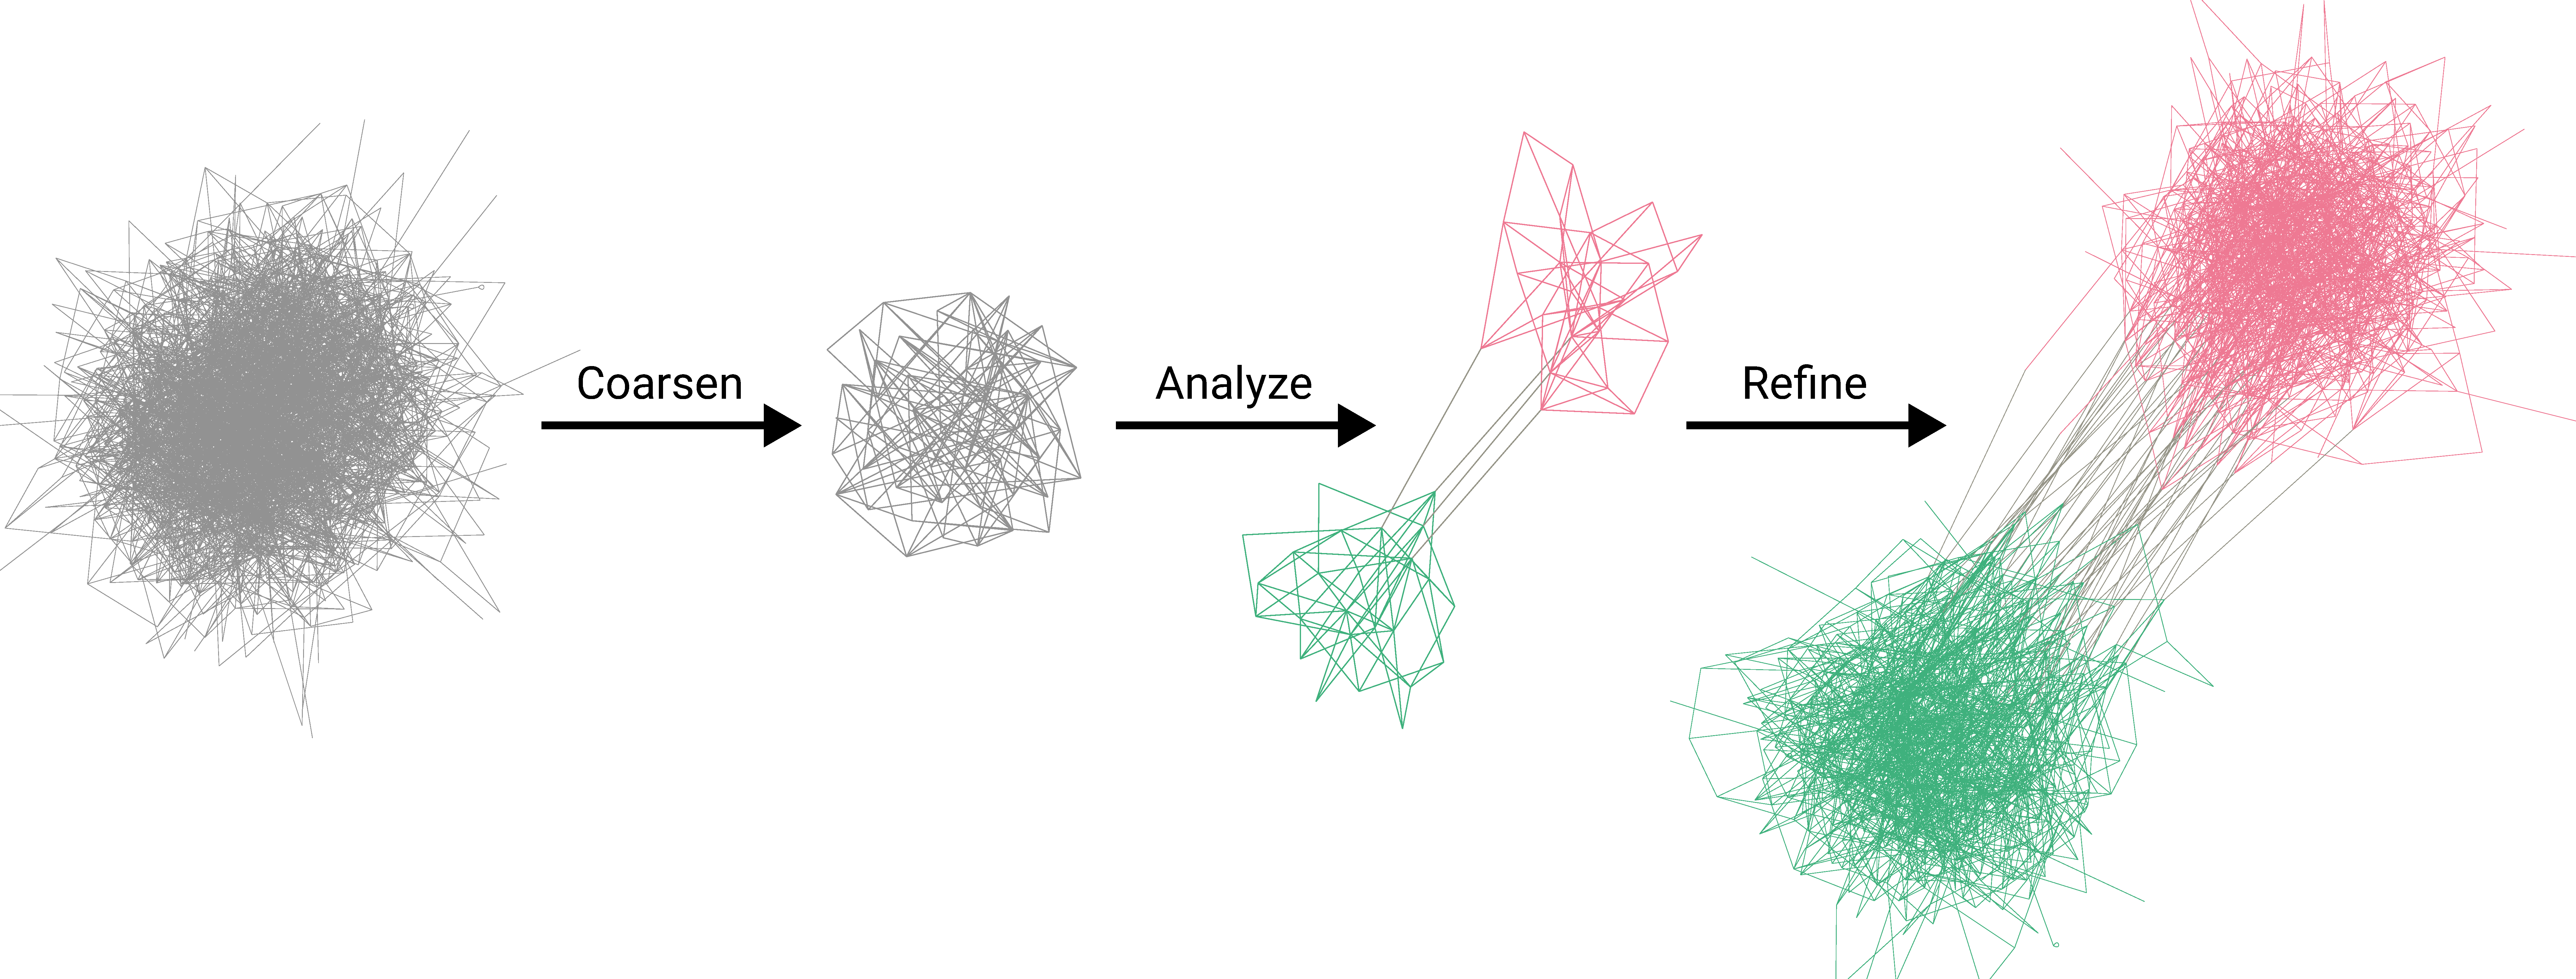
\includegraphics[width=0.8\linewidth]{gfx/intro/overview.pdf}
	\caption{%
		Using graph coarsening to speed up graph algorithms, e.g.\  Min-Cut.
	}\label{fig:intro:overview}
\end{figure}

The goal of this paper is to show how graph coarsening works and how it affects the results of graph algorithms.
This introduction consists of three sections, each of which aims to answer one main question:
\begin{enumerate}
	\item \textit{How can the structural properties of a graph be formally described?}
		To describe graph coarsening and its effects, the similarity between a graph $G$ and its coarsened version $G_c$ has to be quantified.
		We begin with an introduction to spectral graph theory.
		It allows us to describe the structure of graphs and provides the notion of the \textit{graph spectrum}, a way to describe the overall structure of graphs.
	\item \textit{How does graph coarsening work?}
		Based on the notion of the graph spectrum, we will formally define the graph coarsening operation and describe a randomized coarsening algorithm.
	\item \textit{How does coarsening affect the result of graph algorithms?}
		Finally we will put bounds on how much the described coarsening algorithm is expected to increase the error of the spectral clustering algorithm.
\end{enumerate}

% !TEX root = ../main.tex
% chktex-file 21
% chktex-file 46
\section{Conclusion}%
\label{sec:conclusion}

We have now discussed the three main topics of this paper:
\begin{enumerate*}
	\item How the structural properties of graphs can be described via spectral graph theory.
	\item How graphs can be coarsened via the REC algorithm.
	\item How to bound the effects of coarsening via RSS and what this implies for spectral clustering.
\end{enumerate*}

Based on the work we presented, there are two main open questions for future research:
\begin{enumerate*}
	\item The described RSS bound assumes a single application of the REC algorithm.
		For multiple REC applications with a total reduction ratio of $r > \frac{1}{2}$, the RSS bound still needs to be generalized.
	\item Currently the RSS bound has only been applied to the analysis of spectral clustering.
		To make the results more generally applicable, the implications for other graph algorithms, e.g.\ graph convolutional neural networks, are still to be considered.
\end{enumerate*}


% --------------------------
% Back matter
% --------------------------
{%
\renewcommand{\bibfont}{\normalfont\small}
\setlength{\biblabelsep}{5pt}
\setlength{\bibitemsep}{0.5\baselineskip plus 0.5\baselineskip} % chktex 1
\setcounter{biburllcpenalty}{9000}
\setcounter{biburlucpenalty}{9999}
\printbibliography[nottype=www]
\printbibliography[heading=subbibliography,title={Webpages},type=www]
}

% **************************************************
% End of Document CONTENT
% **************************************************
\end{document}
